\chapter{Schedule}
\justify
The duration of this project is a total of 20 weeks. During that time the project team will work on a design for the system and work on a prototype. To make it more clear what is going to happen during that time, a schedule will be created in a form of a Gantt-chart. The schedule will be split into 2 parts for each quarter The schedules can be found in figure \ref{fig:PQ1} and \ref{fig:PQ2}. This chapter will explain more in detail how the schedule is planned.

\section{Quarter 1}
\justify

In the first quarter, the project team will focus on designing a system which meets the requirements of the client. In the first week, the team will make contact with the client and the supervisor of the project. By meeting them, the team can make plans for this project. Meetings with the client and the supervisor will be scheduled weekly to discuss the progress of the project. After this, in the next week a Plan of Approach will be handed to the client. When this is done, the team will have 2 weeks to research each component and make a design for the system, which controls the LIDAR and the camera. If any components are missing or not available, these can be purchased during this time.

\justify
If everything is complete and all components are available, the team can start working on the system. The team will probably be split in 2 groups. One of the groups will start working on setting up the system and the other one will start making a program. When both teams are finished the 2 parts will be combined and the system can be tested. There will be time for this until week 13, because in week 14 the team will be busy with exams of other subjects and will not have much time to work on the project.

\justify
In week 15 an assessment will be organized by the Hague University to review how the project is going and what the progress is of the projects. A extra week is scheduled if any extra time is needed to catch up with the project.

\section{Quarter 2}

In the first quarter the team focused more on the design of the system. If everything went well and the team accomplished on making a working pre-system, a PCB will be designed of the system in the second quarter. The first week will be dedicated to making any changes to the system if anything was not satisfactory to the client. When done with this, the team will start designing the system in the program KiCad. When the design is complete, the components for the PCB will can be purchased and the PCB-design can be send to the manufacturer. Printing the PCB normally takes roughly a week to deliver. When all components have arrived, the project team can start working on soldering the PCB. 

\justify
After completing the PCB, The program made in the previous quarter may need to be adjusted so that the it works with the newly designed PCB. After changing the code of the program, the PCB can be tested with the LIDAR and the camera. The tests will be documented in the final report and the deadline for this is at the end of week 23. Again in week 24, the team has some exams and has little time working on the project. Somewhere in week 25 another assessment will be held and the team will present the final result of the project.

\newpage

\begin{landscape}

\begin{figure}
    \centering
    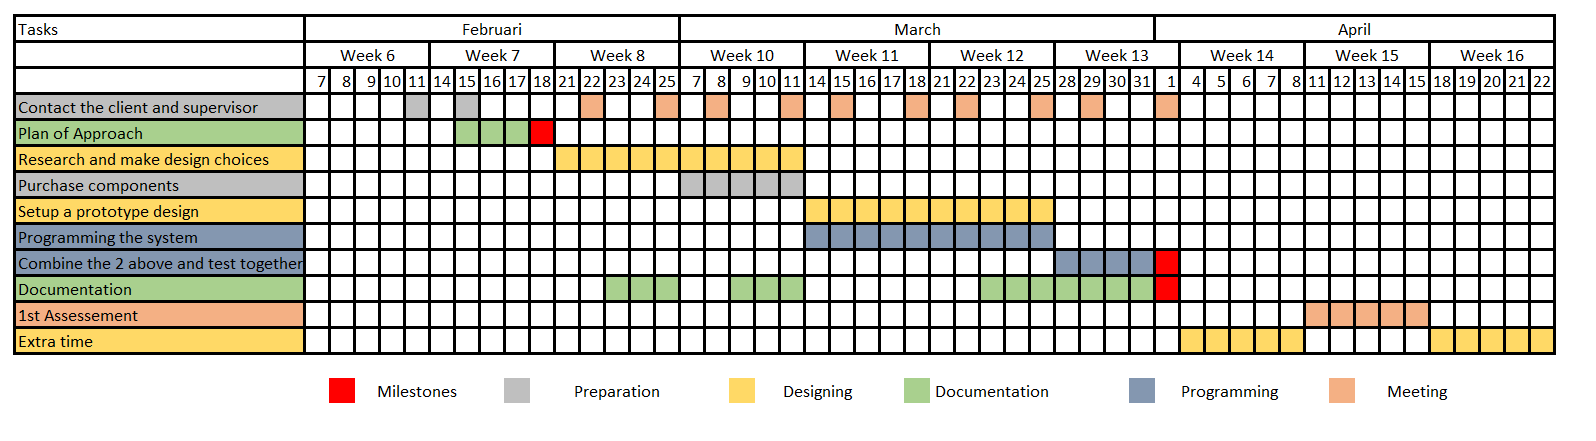
\includegraphics[scale = 0.6]{images/Planning_Lider_Q1.png}
    \caption{Planning Quarter 1}
    \label{fig:PQ1}
\end{figure}

\begin{figure}
    \centering
    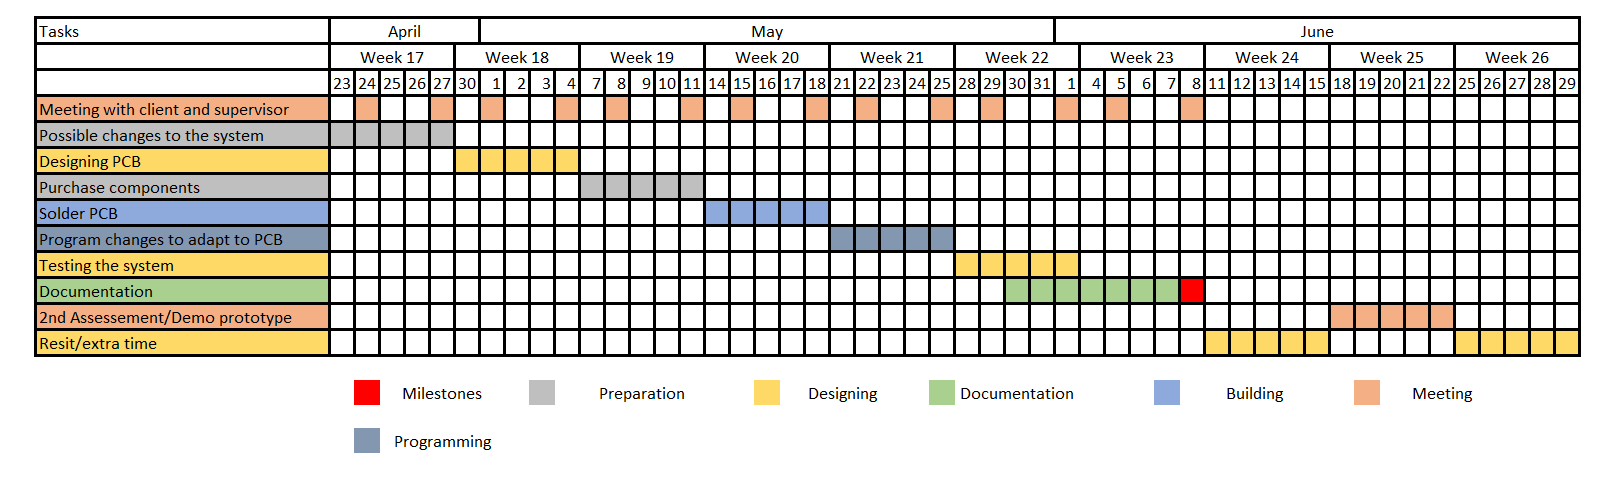
\includegraphics[scale = 0.6]{images/Planning_Lider_Q2.png}
    \caption{Planning Quarter 2}
    \label{fig:PQ2}
\end{figure}

\end{landscape}